\documentclass[12pt]{report}

\usepackage{graphicx}
\graphicspath{ {./images} }

\usepackage{parskip}
\setlength{\parskip}{\baselineskip}
\setlength{\parindent}{0pt}

\title{Jane Goodall Script}
\author{Rayhan \and Odi \and Bagas}

\begin{document}

\maketitle

\centering

\subsection*{Orientation of Jane Goodall}

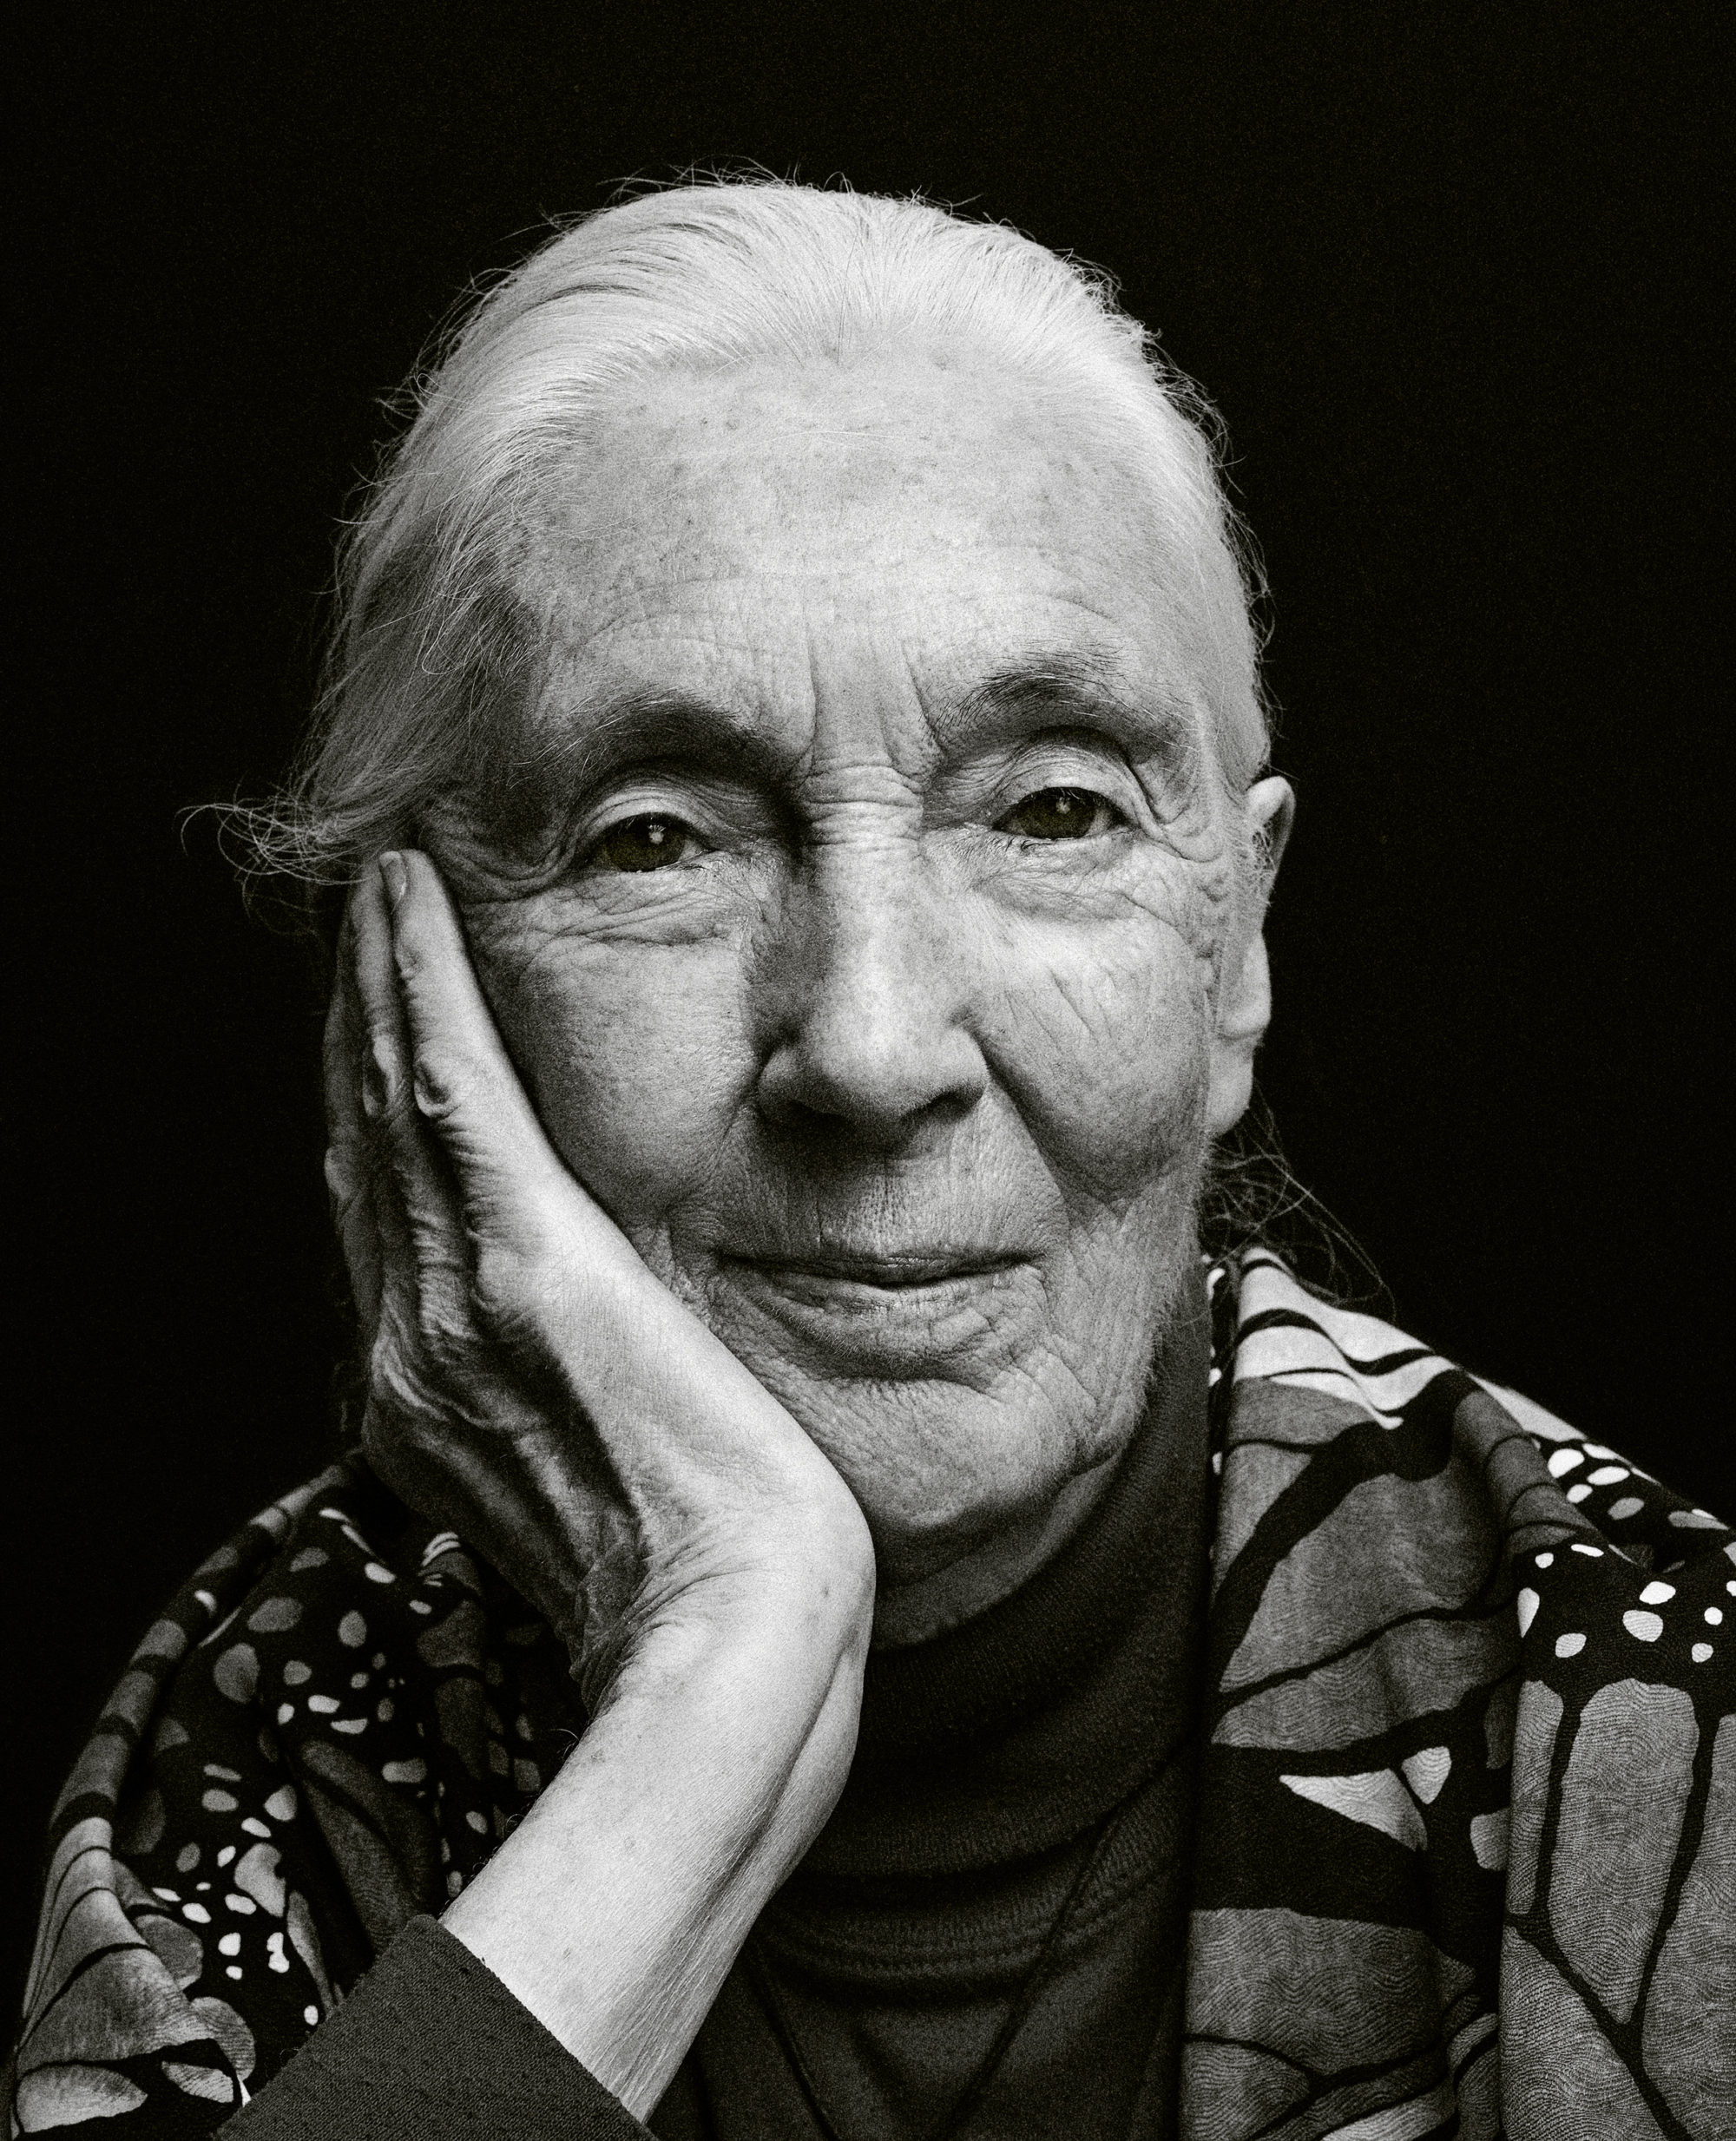
\includegraphics[
    width=5cm,
    height=7cm,
    keepaspectratio
]{jane-goodall-introduction}

Meet Jane Goodall, one of the pioneering English primatologists. Goodall is
well known for her expansive research and dedication in order to save the lives
of chimpanzees around the world.

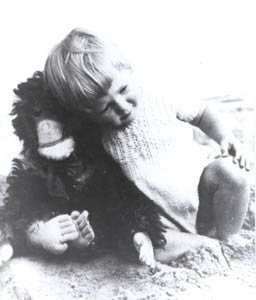
\includegraphics[
    width=6cm,
    height=15cm,
    keepaspectratio
]{jane-goodall-jubilee}

Her sheer passion was all thanks to Jubilee, a chimpanzee doll Goodall acquired
during her first birthday. This was what sparked Goodall's unadulterated
fascination with chimpanzees.

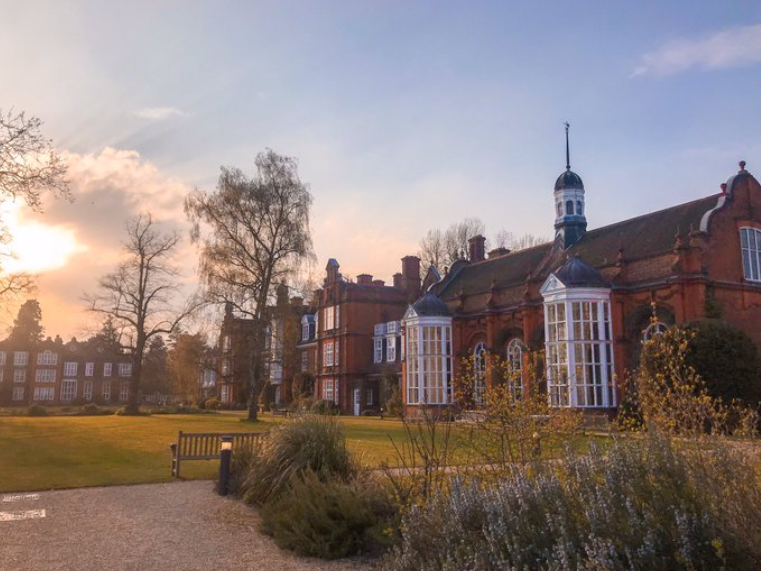
\includegraphics[
    width=10cm,
    height=18cm,
    keepaspectratio
]{newnham-college}

For university, Goodall first went to Newnham College, where she eventually
received her Bachelor of Arts in natural sciences.

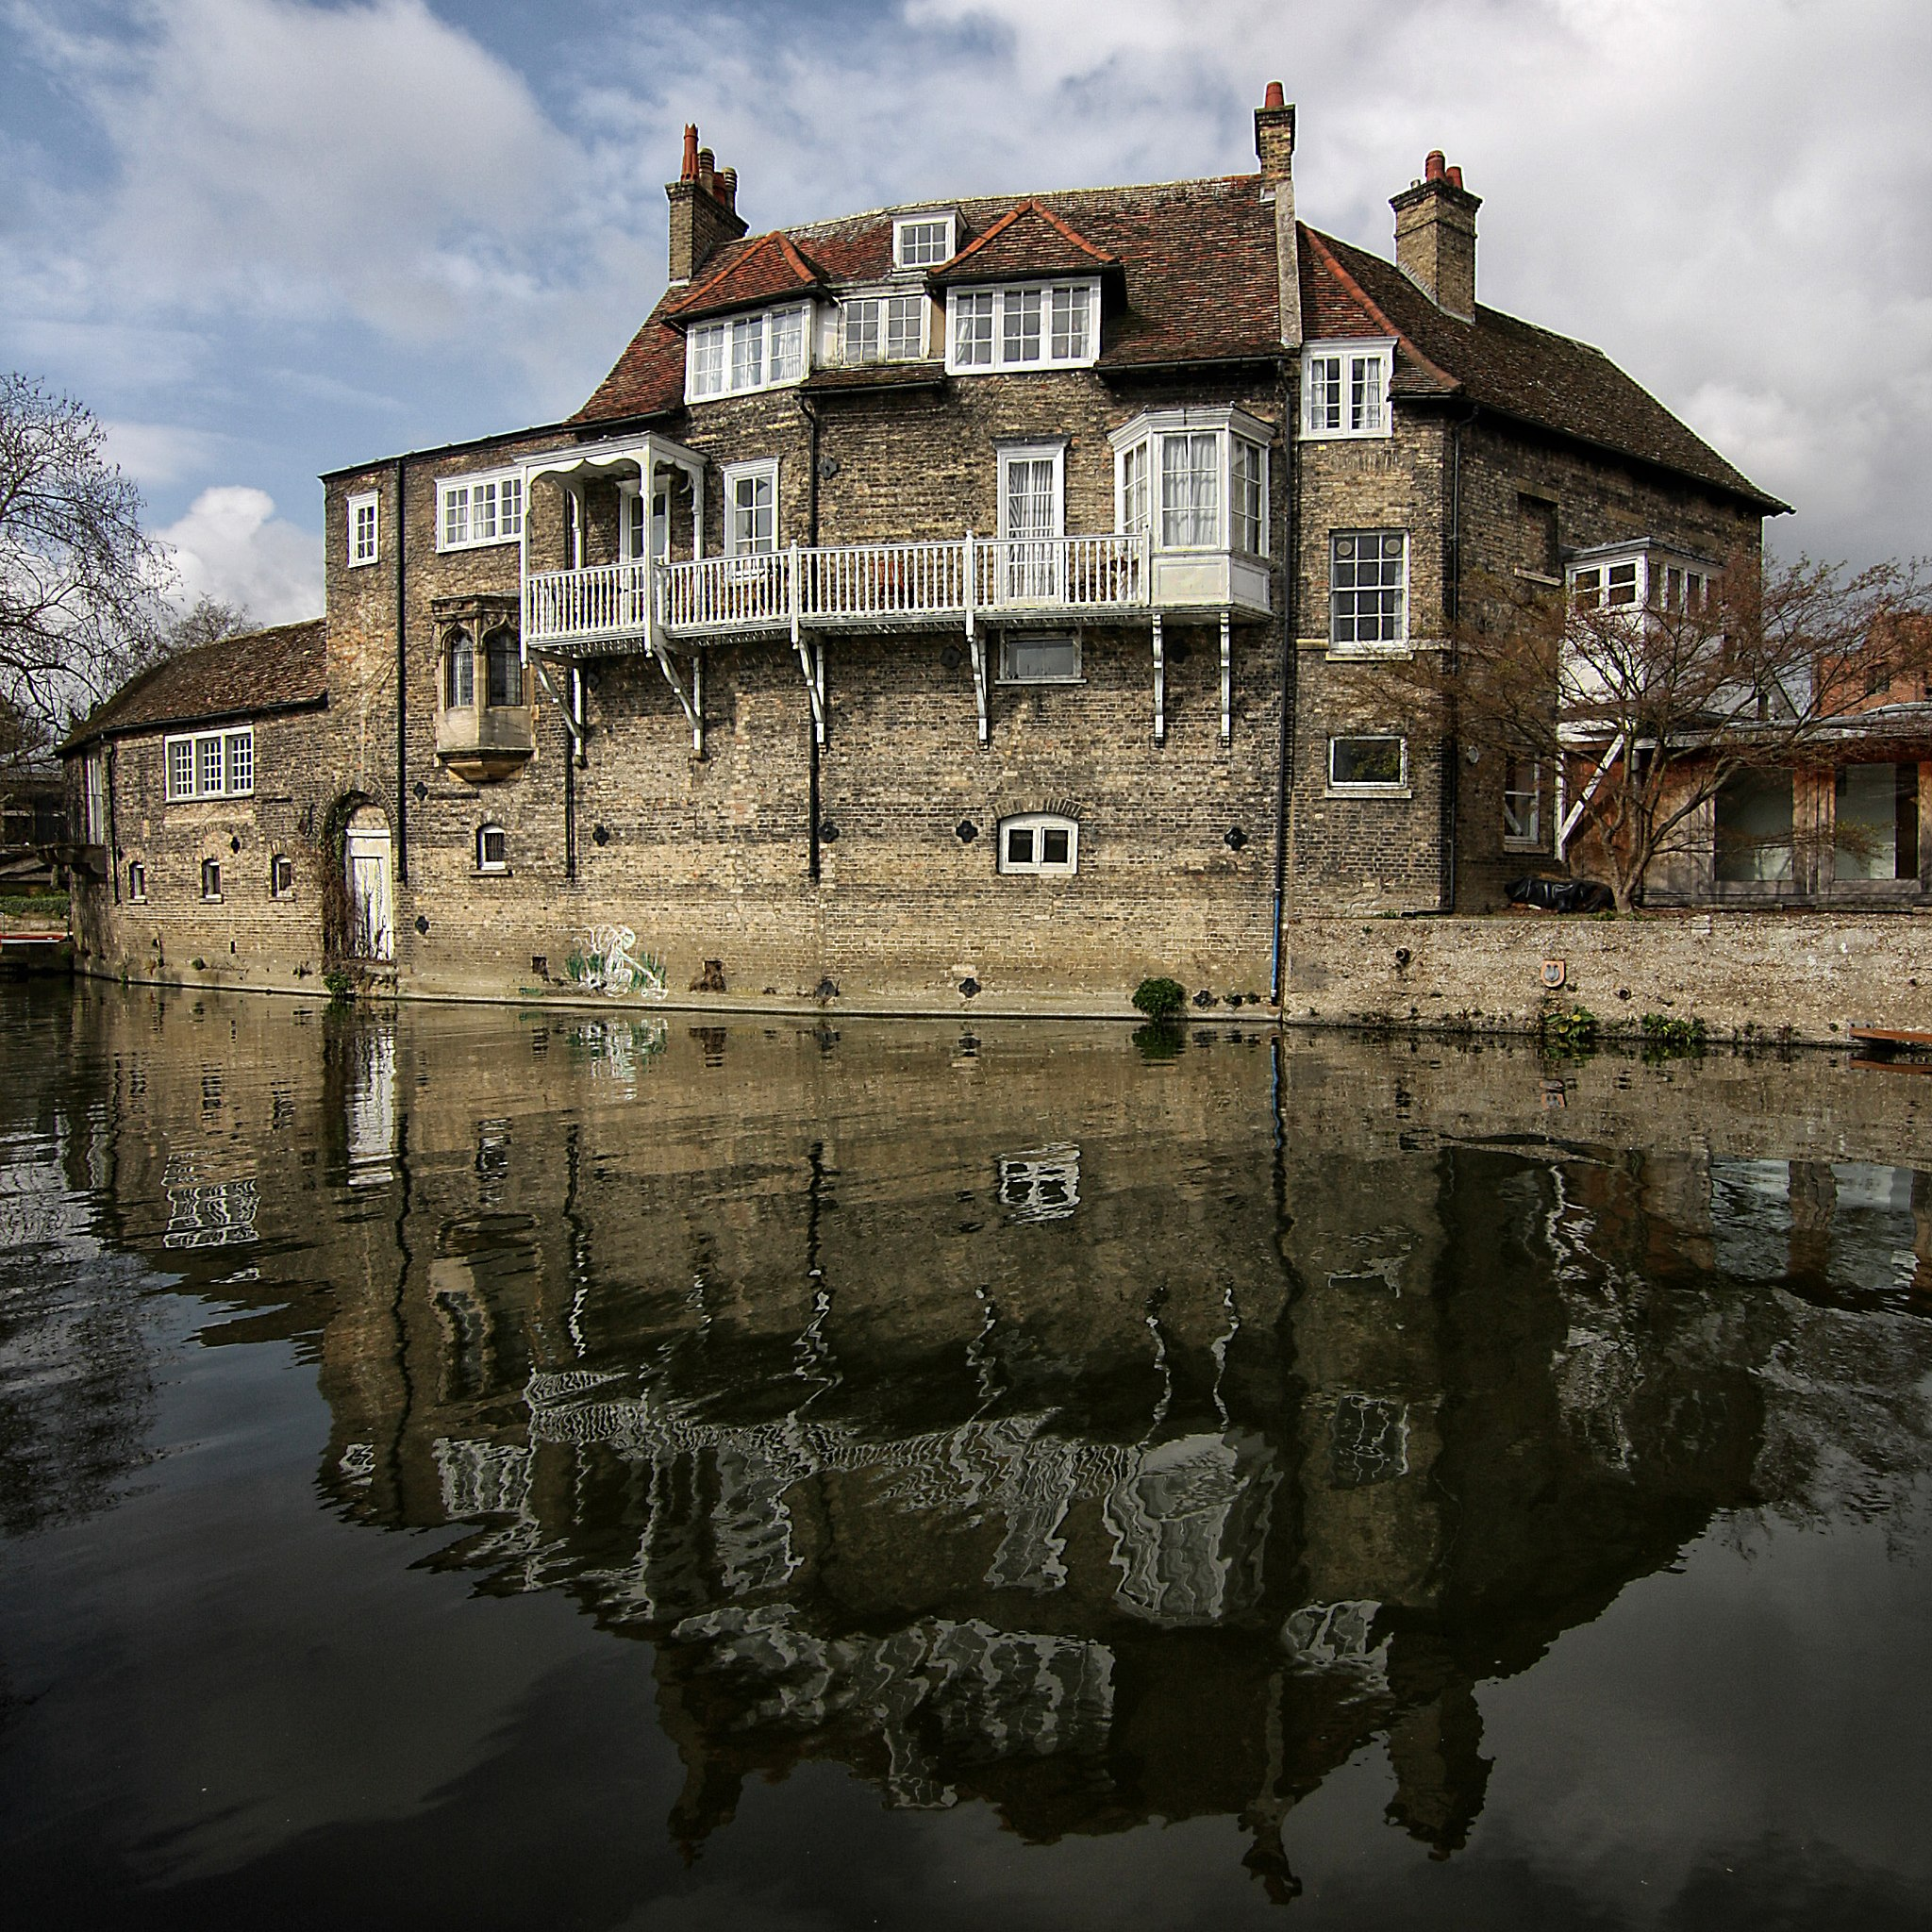
\includegraphics[
    width=8cm,
    height=18cm,
    keepaspectratio
]{darwin-college}

And that is when she attended Darwin College, aiming for a Doctor of Philosophy
in ethology.

\end{document}
